\documentclass[tikz, border=14pt]{standalone}
\usepackage{tikz}
\usetikzlibrary{arrows.meta, calc, positioning}

% ─── Color palette ────────────────────────────────────────────────────────────
\definecolor{ubcfill}{RGB}{222, 218, 210}
\definecolor{ubcstroke}{RGB}{152, 147, 140}
\definecolor{ubcedgecol}{RGB}{186, 181, 173}
\definecolor{treatA}{RGB}{38, 82, 200}
\definecolor{treatB}{RGB}{208, 50, 50}
\definecolor{sharedcol}{RGB}{110, 98, 172}
\definecolor{targetcol}{RGB}{42, 132, 76}
\definecolor{targetstroke}{RGB}{28, 95, 54}

% ─── Styles ───────────────────────────────────────────────────────────────────
\tikzset{
  ubc/.style={circle, draw=ubcstroke, fill=ubcfill, minimum size=7pt, inner sep=0pt, line width=0.6pt},
  ubc1/.style={ubc, fill=ubcfill!80!white, draw=ubcstroke!75!white},
  ubc2/.style={ubc, fill=ubcfill!58!white, draw=ubcstroke!53!white},
  ubc3/.style={ubc, fill=ubcfill!36!white, draw=ubcstroke!32!white},
  ubc4/.style={ubc, fill=ubcfill!22!white, draw=ubcstroke!18!white},
  ubcP/.style={ubc, fill=ubcfill!12!white, draw=ubcstroke!10!white},
  nodeA/.style={ubc, draw=treatA!70!black, fill=treatA!18!white, line width=0.8pt},
  nodeB/.style={ubc, draw=treatB!70!black, fill=treatB!18!white, line width=0.8pt},
  nodeAB/.style={ubc, draw=sharedcol!75!black, fill=sharedcol!20!white, line width=0.8pt},
  target/.style={circle, draw=targetstroke, fill=targetcol, minimum size=13pt, inner sep=0pt, line width=1.0pt, text=white, font=\scriptsize\bfseries},
  ubc edge/.style={-Stealth, color=ubcedgecol, line width=0.6pt, shorten >=2pt, shorten <=2pt},
  ubc1 edge/.style={ubc edge, color=ubcedgecol!80!white},
  ubc2 edge/.style={ubc edge, color=ubcedgecol!58!white},
  ubc3 edge/.style={ubc edge, color=ubcedgecol!36!white},
  ubc4 edge/.style={ubc edge, color=ubcedgecol!22!white},
  ubcP edge/.style={ubc edge, color=ubcedgecol!12!white},
  ubc stub/.style={color=ubcedgecol, line width=0.5pt, shorten <=2pt},
  ubc1 stub/.style={ubc stub, color=ubcedgecol!80!white},
  ubc2 stub/.style={ubc stub, color=ubcedgecol!58!white},
  ubc3 stub/.style={ubc stub, color=ubcedgecol!36!white},
  ubc4 stub/.style={ubc stub, color=ubcedgecol!22!white},
  ubcP stub/.style={ubc stub, color=ubcedgecol!12!white},
  treatA edge/.style={-latex, color=treatA, line width=0.8pt, opacity=1.0, shorten >=3pt, shorten <=3pt},
  treatB edge/.style={-latex, color=treatB, line width=0.8pt, opacity=1.0, shorten >=3pt, shorten <=3pt},
  shared edge/.style={-latex, color=sharedcol, line width=1.5pt, opacity=1.0, shorten >=3pt, shorten <=3pt},
  ingrA/.style={-latex, color=treatA, line width=1.0pt, dash pattern=on \pgflinewidth off 1.75pt, line cap=round, shorten >=3pt},
  ingrB/.style={-latex, color=treatB, line width=1.0pt, dash pattern=on \pgflinewidth off 1.75pt, line cap=round, shorten >=3pt},
}

\begin{document}
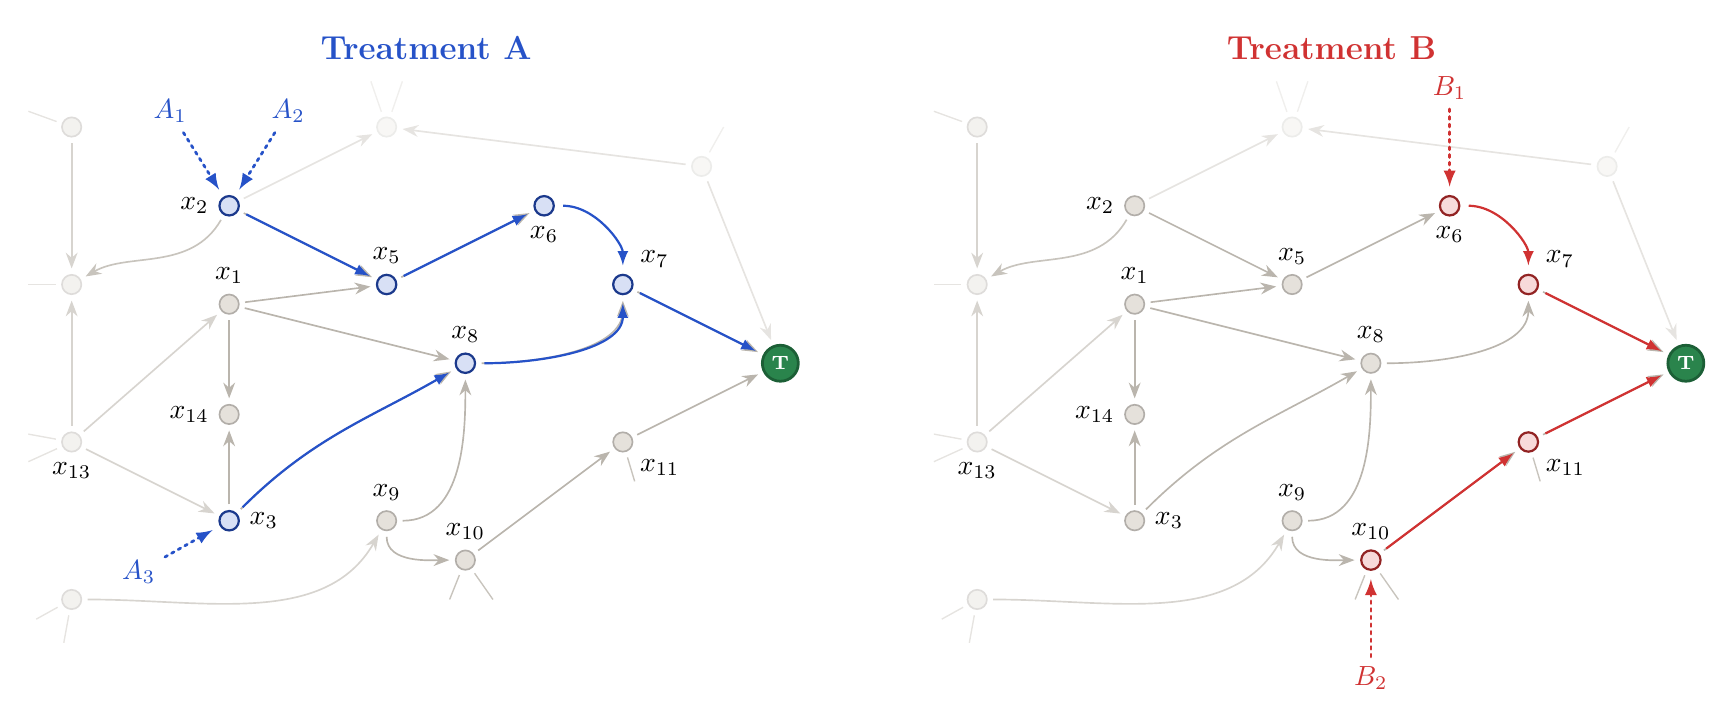
\begin{tikzpicture}[x=1cm, y=1cm]

  %% ── Treatment A ─────────────────────────────────────────────────────────────
  \begin{scope}[name prefix=A-]
    \node[ubc1, label={above:$x_1$}]            (x1)  at (0.0,  0.75) {};
    \node[nodeA, label={left:$x_2$}]            (x2)  at (0.0,  2.0)  {};
    \node[nodeA, label={right:$x_3$}]           (x3)  at (0.0, -2.0)  {};
    \node[nodeA, label={above:$x_5$}]           (x5)  at (2.0,  1.0)  {};
    \node[nodeA, label={below:$x_6$}]           (x6)  at (4.0,  2.0)  {};
    \node[nodeA, label={above right:$x_7$}]     (x7)  at (5.0,  1.0)  {};
    \node[nodeA, label={above:$x_8$}]           (x8)  at (3.0,  0.0)  {};
    \node[ubc1, label={above:$x_9$}]            (x9)  at (2.0, -2.0)  {};
    \node[ubc1, label={above:$x_{10}$}]         (x10) at (3.0, -2.5)  {};
    \node[ubc1, label={below right:$x_{11}$}]   (x11) at (5.0, -1.0)  {};
    \node[ubc1, label={left:$x_{14}$}]          (x14) at (0.0, -0.65) {};
    \node[ubc3] (x12) at (-2.0, -3.0) {};
    \node[ubc3, label={below:$x_{13}$}] (x13) at (-2.0, -1.0) {};
    \node[ubc3] (x15) at (-2.0,  1.0) {};
    \node[ubc3] (x16) at (-2.0,  3.0) {};
    \node[ubc4] (x4)  at ( 2.0,  3.0) {};
    \node[ubc4] (x18) at ( 6.0,  2.5) {};
    \node[font=\large\bfseries, color=treatA] at (2.5, 4.0) {Treatment A};
    \node[font=\bfseries, color=treatA] (nA1) at (-0.75,  3.2)  {$A_1$};
    \node[font=\bfseries, color=treatA] (nA2) at (0.75,  3.2)  {$A_2$};
    \node[font=\bfseries, color=treatA] (nA3) at (-1.15, -2.65)  {$A_3$};
    \node[target] (T) at (7.0, 0) {T};
    \draw[ubc edge]  (x1) -- (x5);    \draw[ubc edge]  (x1) -- (x8);
    \draw[ubc edge]  (x1) -- (x14);
    \draw[ubc3 edge] (x2) -- (x4);    \draw[ubc edge]  (x2) -- (x5);
    \draw[ubc edge]  (x3) to[out=45, in=-150] (x8);
    \draw[ubc edge]  (x3) -- (x14);   \draw[ubc edge]  (x5) -- (x6);
    \draw[ubc edge]  (x8) to[out=0, in=-90] (x7);
    \draw[ubc edge]  (x9) to[out=0, in=-90] (x8);
    \draw[ubc edge]  (x9) to[out=-90, in=180] (x10);
    \draw[ubc edge]  (x10) -- (x11);  \draw[ubc edge]  (x7) -- (T);
    \draw[ubc edge]  (x11) -- (T);    \draw[ubc3 edge] (x18) -- (T);
    \draw[ubc3 edge] (x18) -- (x4);   \draw[ubc1 edge] (x2) to[out=-120, in=30] (x15);
    \draw[ubc2 edge] (x13) -- (x15);  \draw[ubc2 edge] (x16) -- (x15);
    \draw[ubc2 edge] (x12) to[out=0, in=-120] (x9);
    \draw[ubc2 edge] (x13) -- (x1);   \draw[ubc2 edge] (x13) -- (x3);
    \draw[ubc3 stub] (x16) -- +(-0.55,  0.20);  \draw[ubc3 stub] (x15) -- +(-0.55,  0.00);
    \draw[ubc3 stub] (x13) -- +(-0.55,  0.10);  \draw[ubc3 stub] (x13) -- +(-0.55, -0.25);
    \draw[ubc3 stub] (x12) -- +(-0.45, -0.25);  \draw[ubc3 stub] (x12) -- +(-0.10, -0.55);
    \draw[ubc4 stub] (x4)  -- +(-0.20,  0.58);  \draw[ubc4 stub] (x4)  -- +( 0.20,  0.58);
    \draw[ubc4 stub] (x18) -- +( 0.28,  0.50);
    \draw[ubc1 stub] (x10) -- +(-0.20, -0.50);  \draw[ubc1 stub] (x10) -- +( 0.35, -0.50);
    \draw[ubc1 stub] (x11) -- +( 0.15, -0.50);
    \draw[treatA edge] (x2) -- (x5);
    \draw[treatA edge] (x3) to[out=45, in=-150] (x8);
    \draw[treatA edge] (x5) -- (x6);
    \draw[treatA edge] (x6) to[out=0, in=90] (x7);
    \draw[treatA edge] (x8) to[out=0, in=-90] (x7);
    \draw[treatA edge] (x7) -- (T);
    \draw[ingrA] (nA1) -- (x2);
    \draw[ingrA] (nA2) -- (x2);
    \draw[ingrA] (nA3) -- (x3);
  \end{scope}

  %% ── Treatment B ─────────────────────────────────────────────────────────────
  \begin{scope}[name prefix=B-, xshift=11.5cm]
    \node[ubc1, label={above:$x_1$}]            (x1)  at (0.0,  0.75) {};
    \node[ubc1, label={left:$x_2$}]             (x2)  at (0.0,  2.0)  {};
    \node[ubc1, label={right:$x_3$}]            (x3)  at (0.0, -2.0)  {};
    \node[ubc1, label={above:$x_5$}]            (x5)  at (2.0,  1.0)  {};
    \node[nodeB, label={below:$x_6$}]           (x6)  at (4.0,  2.0)  {};
    \node[nodeB, label={above right:$x_7$}]     (x7)  at (5.0,  1.0)  {};
    \node[ubc1, label={above:$x_8$}]            (x8)  at (3.0,  0.0)  {};
    \node[ubc1, label={above:$x_9$}]            (x9)  at (2.0, -2.0)  {};
    \node[nodeB, label={above:$x_{10}$}]        (x10) at (3.0, -2.5)  {};
    \node[nodeB, label={below right:$x_{11}$}]  (x11) at (5.0, -1.0)  {};
    \node[ubc1, label={left:$x_{14}$}]          (x14) at (0.0, -0.65) {};
    \node[ubc3] (x12) at (-2.0, -3.0) {};
    \node[ubc3, label={below:$x_{13}$}] (x13) at (-2.0, -1.0) {};
    \node[ubc3] (x15) at (-2.0,  1.0) {};
    \node[ubc3] (x16) at (-2.0,  3.0) {};
    \node[ubc4] (x4)  at ( 2.0,  3.0) {};
    \node[ubc4] (x18) at ( 6.0,  2.5) {};
    \node[font=\large\bfseries, color=treatB] at (2.5, 4.0) {Treatment B};
    \node[font=\bfseries, color=treatB] (nB1) at (4.0,  3.5)  {$B_1$};
    \node[font=\bfseries, color=treatB] (nB2) at (3.0, -4.0)  {$B_2$};
    \node[target] (T) at (7.0, 0) {T};
    \draw[ubc edge]  (x1) -- (x5);    \draw[ubc edge]  (x1) -- (x8);
    \draw[ubc edge]  (x1) -- (x14);
    \draw[ubc3 edge] (x2) -- (x4);    \draw[ubc edge]  (x2) -- (x5);
    \draw[ubc edge]  (x3) to[out=45, in=-150] (x8);
    \draw[ubc edge]  (x3) -- (x14);   \draw[ubc edge]  (x5) -- (x6);
    \draw[ubc edge]  (x8) to[out=0, in=-90] (x7);
    \draw[ubc edge]  (x9) to[out=0, in=-90] (x8);
    \draw[ubc edge]  (x9) to[out=-90, in=180] (x10);
    \draw[ubc edge]  (x10) -- (x11);  \draw[ubc edge]  (x7) -- (T);
    \draw[ubc edge]  (x11) -- (T);    \draw[ubc3 edge] (x18) -- (T);
    \draw[ubc3 edge] (x18) -- (x4);   \draw[ubc1 edge] (x2) to[out=-120, in=30] (x15);
    \draw[ubc2 edge] (x13) -- (x15);  \draw[ubc2 edge] (x16) -- (x15);
    \draw[ubc2 edge] (x12) to[out=0, in=-120] (x9);
    \draw[ubc2 edge] (x13) -- (x1);   \draw[ubc2 edge] (x13) -- (x3);
    \draw[ubc3 stub] (x16) -- +(-0.55,  0.20);  \draw[ubc3 stub] (x15) -- +(-0.55,  0.00);
    \draw[ubc3 stub] (x13) -- +(-0.55,  0.10);  \draw[ubc3 stub] (x13) -- +(-0.55, -0.25);
    \draw[ubc3 stub] (x12) -- +(-0.45, -0.25);  \draw[ubc3 stub] (x12) -- +(-0.10, -0.55);
    \draw[ubc4 stub] (x4)  -- +(-0.20,  0.58);  \draw[ubc4 stub] (x4)  -- +( 0.20,  0.58);
    \draw[ubc4 stub] (x18) -- +( 0.28,  0.50);
    \draw[ubc1 stub] (x10) -- +(-0.20, -0.50);  \draw[ubc1 stub] (x10) -- +( 0.35, -0.50);
    \draw[ubc1 stub] (x11) -- +( 0.15, -0.50);
    \draw[treatB edge] (x10) -- (x11);
    \draw[treatB edge] (x11) -- (T);
    \draw[treatB edge] (x6) to[out=0, in=90] (x7);
    \draw[treatB edge] (x7) -- (T);
    \draw[ingrB] (nB1) -- (x6);
    \draw[ingrB] (nB2) -- (x10);
  \end{scope}

\end{tikzpicture}
\end{document}